\subsection{Konzeptionelle und Organisatorische Aufgaben}
In diesem Abschnitt finden sich Aufgaben konzeptioneller sowie organisatorischer Natur, die sich mit dem Software-Entwicklungsprozess beschäftigt haben.

\subsubsection{Pflege eines schemenhaften Klassendiagramms}
Um die Struktur unseres Programmes grob zu visualisieren und so eine bessere Orientierung im Code zu ermöglichen sowie einen einheitlichen Wissensstand unter allen Beteiligten zu etablieren, erarbeitete und pflegte Felix Baumgarten ein Klassendiagramm.
Dieses half unter anderem, die Aufgabenverteilung mittels Git-Branches und die Kapselungsorganisation zu vereinfachen. Während der Arbeit am Projekt wurde das Diagramm an einem Whiteboard abgebildet und ergänzt, da Änderungen schnell umzusetzen waren und wir uns Einarbeitungszeit in komplexere digitale UML-Diagramme sparen wollten.
Eine Skizze des deutlich detaillierteren, da unter anderem mit Kardinalitäten ausgestatteten Klassendiagrams:
\begin{figure}
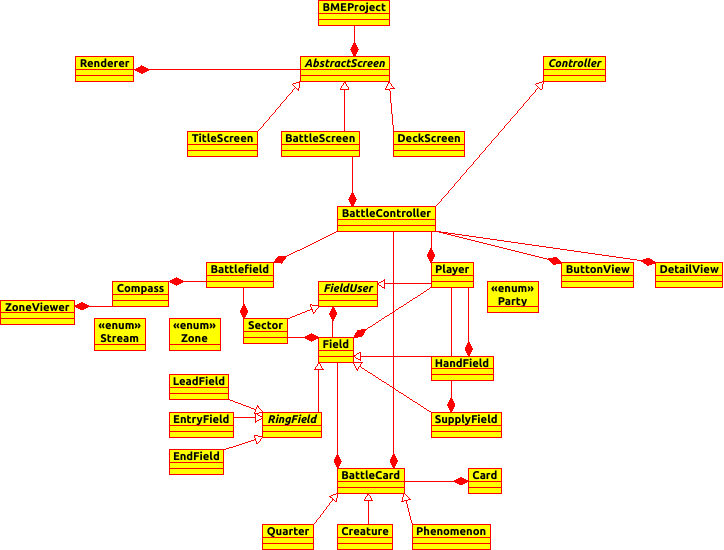
\includegraphics[width=1\textwidth]{../img/klassendiagramm.PNG}
\caption{Klassendiagramm Edwards Biotope}
\label{fig:Klassendiagramm_Edwards_Biotope}
\end{figure}


\subsubsection{Merging und Abnahme}
Im letzten Abschnitt dieses Semesters wurde der Abnahme Prozess innerhalb des Projektsteams nocheinmal überarbeitet.
Ziel war es dieses Semester alle Teammitglieder stärker in die konkrete Implementation von Anforderungen einzubeziehen. Unser ursprüngliches Herangehen war es, dass pro Branch bis zu drei Personen ein Review durchführen und dem jeweiligen Entwickler Feedback und ggf. Korrekturen mitteilen, die an dem Branch vorzunehmen sind. Dies erwies sich fortschreitend als ein Flaschenhals in dem Vorgehen. Der Zeitaufwand der nötig war um mehrere Personen in ein solches Review für jeden einzelnen Branch zu involvieren sorgte für fortschreitend starke Verzögerungen was die Aktuallisierung unserers Develop-Standes anging. Das wiederum sorgte entsprechend dafür, dass gewisse Anforderungen, die auf anderen Anforderungen basierten, nicht umgesetzt werden konnten, bis eben diese Aktuallisierung stattfand. Wir entschieden uns entsprechend dafür, dass Sebastian Beck und Philadelphia Gauss für die Abnahme und das Merging der Branches zuständig waren und das als eine ihrer Hauptaufgaben behandeln. 
Damit strukturierte sich der Prozess nun neu, wie folgt:
\begin{itemize}
\item Erstellung eines Branches ab Develop (durch Entwickler oder einer der beiden Verantwortlichen)
\item Implementation des jeweliligen Branches anhand der Anforderung die entweder im Glo-Board, Teammeeting oder beim Coding-Treffen definiert wurde
\item Erstellen eines Pull-Requests mit Reviewer Sebastian Beck oder Philadelphia Gaus 
\end{itemize}
Ab hier begann der Review-Prozess, der sich wie folgt gliederte:
\begin{itemize}
\item Checktout des jeweiligen Branches
\item Erstes Build lokal und erster manueller Test ob Funktionalität umgestzt wurde
\item einfaches Code-Review
\item bei größeren Fehlern oder nötigen Anpassungen: Rückmeldung an den Entwickler, sonst kleinere Korrekturen durch Reviewer
\item Prüfung ob Merge-Konflikte bestehen und diese ggf. beheben
\item Erneute Prüfung der Lauffähigkeit
\item Abschließender Merge nach Develop
\end{itemize}
Gerade nach der Korrektur von Merge-Konflikten fiel, vorallem bei komplexen Änderungen, immer wieder auf, dass der mitglieferte Diff-Editor von Gitkraken sich nicht immer intuitiv verhielt. Das führte dazu, dass z. T. Methoden automatisiert oder unabsichtlich ineinander verschoben wurden oder nach dem Merge fehlten. Daraufhin führten wir vorallem bei umfangreichen Änderungen mit ein, dass der Stand nach Konfliktbehebung mittels dem Tool "Meld" \cite{Meld} erneut mit dem zu mergenden Stand abgeglichen wurde. Meld ermöglicht es relativ einfach komplette Verzeichnisse miteinander zu vergleichen und auf Unterschiede zu untersuchen. Damit konnten wir fehlenden Code oder fehlende Änderungen weitestgehend auszuschließen. Hierfür musste das Repository lediglich ein zweites mal in ein weiteres Verzeichnis ausgecheckt werden um die beiden Branches über Meld miteinander zu vergleichen. Im diesem Zuge wurde kurz auch das Tool "xxdiff" betrachtet, Meld wurde jedoch abschließend aufgrund seines einfachen UI bevorzugt. \\
Das beseitigen der Konflikte erfolgte in der Regel über einen Merge des aktuellen Develop-Stands in den jeweilgen Feature-Branch. Anhand dessen wurden die nötigen Korrekturen vorgenommen um die Lauffähigkeit wieder herzustellen. Der neue Stand des Features-Branches konnte nun zurück nach Develop gemerged werden. 

\subsubsection{Ermittlung von Anforderungen}
Im Projektverlauf wurde immer wieder klar, dass gewisse Features zu viel Zeit kosten würden um diese umzusetzen, jedoch nicht zu den Kernmechaniken unseres Spiels beitragen würden.
Auf Basis dessen erstellte Robert Sabo ein Umfangreiches Dokument, welches mit bildern Illustrierte Spielzüge und kurze Texte hierzu auswies. Hierbei handelte es sich um die eben notwendigen Funktionalitäten um unser Spiel spielbar zu machen. Sebastian Beck übernahm in dem Zuge die Aufgabe, die einzelnen Spielschritte zu überprüfen und dabei Objekte, Aktionen und Attribute zu analysieren um eine Basis für die Planung der nächsten Features zu schaffen.

Hier ein exemplarischer Auszug für das Objekt Spieler:
\begin{itemize}
\item Spieler legt Karte auf das Feld.
\item Spieler zieht Karten von seinem Deck.
\item Spielder beendet die Runde.
\item Spieler legt Karte auf ein Eintrittsfeld eines Quartiers auf dem Feld.
\item Spieler aktiviert Farbzone des Farbrads
\end{itemize}

Hieraus lassen sich weitere Objekte wie z. B. "Karte" oder "Feld" identifizieren und weiterentwickeln. Das entsprechende Dokument befindet sich im Anhang "Anforderungen\_Präsentation.docx".
